\documentclass{article}
\usepackage{amsmath}
\usepackage{amssymb}
\usepackage{graphicx}
\usepackage{tikz}
\usetikzlibrary{bayesnet}
\usepackage{hyperref}
\graphicspath{ {./} }
\usepackage{listings}
\usepackage{color}
\usepackage{amsmath}
\usepackage{amssymb}
\usepackage{amsmath}
\usepackage{algorithm}
\usepackage[noend]{algpseudocode}
\usepackage{float}

\definecolor{dkgreen}{rgb}{0,0.6,0}
\definecolor{gray}{rgb}{0.5,0.5,0.5}
\definecolor{mauve}{rgb}{0.58,0,0.82}

\begin{document}

\title{Advanced Machine Learning, Final Project. Model Inference.}

\maketitle

\section*{Model}

We begin by presenting the graphical model corresponding to group factor analysis:

\bigskip

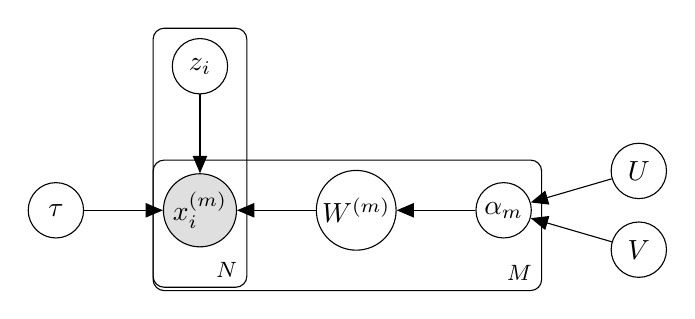
\begin{tikzpicture}

  % Define nodes

  \node[obs] (xi) {$x_i^{(m)}$};
  \node[latent, above=of xi] (zi) {$z_i$};
  \node[latent, left=of xi] (tau) {$\tau$};
  \node[latent, right=of xi] (Wm) {$W^{(m)}$};
  \node[latent, right=of Wm] (alpham) {$\alpha_m$};
  \node[latent, right=of alpham, yshift=0.5 cm] (U) {$U$};
  \node[latent, right=of alpham, yshift=-0.5 cm] (V) {$V$};

  % Connect the nodes
  \edge {zi} {xi};
  \edge {tau} {xi};
  \edge {Wm} {xi};
  \edge {alpham} {Wm};
  \edge {U,V} {alpham};

  % Plates
  \plate {N} {(xi)(zi)} {$N$};
  \plate {M} {(xi)(Wm)(alpham)} {$M$};

\end{tikzpicture}

\bigskip

\begin{description}

\item Where:

\item $X \in \mathbb{R}^{N \times D}$ such that:

	\begin{description}
	\item $X = [X^{(1)},...,X^{(M)}]$
	\item $X^{(m)\intercal} = [x_1^{(m)},...,x_N^{(m)}]$
	\item $p(X|W,Z,\tau) = \prod_i{\prod_m{\mathcal{N}(x_i^{(m)}|W^{(m)\intercal}z_i, \tau_m^{-1}\textbf{I})}}$
	\end{description}

\item $\tau \in \mathbb{R}^{1 \times M}$ such that:

	\begin{description}
	\item $\tau = [\tau_1,...,\tau_M]$
	\item $p(\tau) = \prod_m{\mathcal{G}(\tau_m|a^\tau=10^{-14}, b^\tau=10^{-14})}$
	\end{description}

\item $Z \in \mathbb{R}^{N \times K}$ such that:

	\begin{description}
	\item $Z^\intercal = [z_1,...,z_N]$
	\item $p(Z) = \prod_i{\mathcal{N}(z_i|\textbf{0}, \textbf{1})}$
	\end{description}

\item $W \in \mathbb{R}^{K \times D}$ such that:

	\begin{description}
	\item $W = [W^{(1)},...,W^{(M)}]$
	\item $W^{(m)\intercal} = [w_1^{(m)},...,w_K^{(m)}]$
	\item $w_k^{(m)} \in \mathbb{R}^{D_m}$
	\item $\sum_{m=1}^M{D_m} = D$
	\item $p(W|\alpha) = \prod_{m=1}^M{\prod_{k=1}^K{\prod_{d=1}^{D_m}{\mathcal{N}(w_{k,d}^{(m)}|0, \alpha_{m,k}^{-1})}}}$
	\end{description}

\item $\alpha \in \mathbb{R}^{M \times K}$ such that:
	
	\begin{description}
	\item$log(\alpha) = UV^\intercal + \mu_u \textbf{1}^\intercal + \textbf{1}\mu_v^\intercal$.
	\end{description}

\item $U \in \mathbb{R}^{M \times R}$
	\begin{description}
	\item $p(U) = \prod_m^M{\prod_r^R{\mathcal{N}(u_{m,r}|0, (\lambda=0.1)^{-1})}}$
	\end{description}
\item $V \in \mathbb{R}^{K \times R}$
	\begin{description}
	\item $p(V) = \prod_k^K{\prod_r^R{\mathcal{N}(v_{k,r}|0, (\lambda=0.1)^{-1})}}$
	\end{description}

\end{description}

\bigskip

Then the model's full joint probability can be written as:

$$p(\Theta,X) = p(Z,W,\tau,U,V,X) = p(Z)p(W|\alpha)p(\tau)p(U)p(V)p(X|W,Z,\tau)$$

\section*{Inference}

In order to minimize the Kullback-Leibler divergence:

$$D_{KL}(q||p) = \int_\Theta{q(\Theta)log(\frac{q(\Theta)}{p(\Theta|X)})d\Theta}$$

or equivalently to maximize the lower bound:

$$\mathcal{L}(\Theta) = \int_\Theta{q(\Theta)log(\frac{p(\Theta,X)}{q(\Theta)})d\Theta}$$

We assume:

$$q(\Theta) = q(Z)q(W)q(\tau)q(U)q(V)$$

In which case and by means of variational calculus we must have that $q(\theta_i)$ must have the form:

$$q(\theta_i) = \frac{e^{E_{i\neq j}[log(p(\Theta,X))]}}{\int{e^{E_{i\neq j}[log(p(\Theta,X))]}d\theta_i}}$$

$$\implies log(q(\theta_i)) = E_{i\neq j}[log(p(\Theta,X))] + constant$$

\bigskip

And so we proceed by taking the corresponding expectations with respect to the log of the model's full joint probability:

	
$$log(q(Z)) = E_{W,\tau}[log(p(\Theta,X))]  = E_{W,\tau}[log(p(Z))] + E_{W,\tau}[log(p(X|W,Z,\tau))] + C_1$$

$$ = E_{W,\tau}\bigg[\sum_i^N{log(\mathcal{N}(z_i|\textbf{0}, \textbf{I})})\bigg] + E_{W,\tau}\bigg[\sum_i^N{\sum_m^M{log(\mathcal{N}(x_i^{(m)}|W^{(m)\intercal}z_i, \tau_m^{-1}\textbf{I}))}}\bigg] + C_1$$

$$ = -\frac{1}{2}\sum_i^N{z_i^\intercal z_i -\frac{1}{2}\sum_m^M{E_{W,\tau}\bigg[\tau_m(x_i^{(m)} - W^{(m)\intercal}z_i)^\intercal(x_i^{(m)} - W^{(m)\intercal}z_i) \bigg]}} + C_2$$

$$ = -\frac{1}{2}\sum_i^N{z_i^\intercal \textbf{I}_k z_i + \sum_m^M{\langle\tau_m\rangle(z_i^\intercal \langle W^{(m)}\rangle x_i^{(m)} -\frac{1}{2} z_i^\intercal \langle W^{(m)}W^{(m)\intercal}\rangle z_i)}} + C_3$$

$$ = \sum_i^N{\sum_m^M{z_i^\intercal \langle W^{(m)}\rangle \langle\tau_m\rangle x_i^{(m)} - -\frac{1}{2}z_i^\intercal (\textbf{I}_k + \sum_m^M{\langle\tau_m\rangle \langle W^{(m)}W^{(m)\intercal}\rangle} )z_i}} + C_3$$

Note that above we denote the first moment by $E_{\theta_i}[\theta_i] = \langle \theta_i \rangle$ and the second moment by $E_{\theta_i}[\theta_i \theta_i^\intercal] = \langle \theta_i \theta_i^\intercal \rangle$. Note as well that we collect all constant factors with respect to $z_i$ into $C_1$, $C_2$ and $C_3$ respectively. Then recalling:

$$\mathcal{N}(x|\mu,\Sigma) \propto x^\intercal \Sigma^{-1} \mu - \frac{1}{2} x^\intercal \Sigma^{-1} x$$

We must have:

$$q(Z) = \prod_i^N{\mathcal{N}(m_i^{(z)},\Sigma^{(z)})}$$

with:

$$\Sigma^{(z)} = \bigg(\textbf{I}_k + \sum_m^M{\langle\tau_m\rangle \langle W^{(m)}W^{(m)\intercal}\rangle} \bigg)^{-1}$$

$$m_i^{(z)} = \Sigma^{(z)} \langle W^{(m)}\rangle \langle\tau_m\rangle x_i^{(m)}$$

\bigskip

Similarly we proceed with $q(W)$ in which case we have:

$$log(q(W)) = E_{\alpha,Z,\tau}[log(p(\Theta,X))] = E_{\alpha,Z,\tau}[log(p(W|\alpha))] + E_{\alpha,Z,\tau}[log(p(X|W,Z,\tau))] + C_1$$

$$=E_{\alpha,Z,\tau}\bigg[\sum_{m}^M{\sum_{k}^K{\sum_{d}^{D_m}{log(\mathcal{N}(w_{k,d}^{(m)}|0, \alpha_{m,k}^{-1}))}}}\bigg] + E_{\alpha,Z,\tau}\bigg[\sum_i^N{\sum_m^M{log(\mathcal{N}(x_i^{(m)}|W^{(m)\intercal}z_i, \tau_m^{-1}\textbf{I}))}}\bigg] + C_1$$

We continue by looking at the group columns $w_{:,d}^{(m)}$ in $W$ as opposed to the group rows $w_k^{(m)}$ such that $W^{(m)} = [w_{:,1}^{(m)},...,w_{:,D_m}^{(m)}]$. Then note that the number of columns in $X$ is equal to the number of columns in $W$ and so we have:

$$=E_{\alpha,Z,\tau}\bigg[\sum_{m}^M{\sum_{d}^{D_m}{log(\mathcal{N}(w_{:,d}^{(m)}|\textbf{0}, \overline{\overline{\alpha}}_m^{-1}))}}\bigg] + E_{\alpha,Z,\tau}\bigg[\sum_m^M{\sum_d^{D_m}{\sum_i^N{log(\mathcal{N}(x_{i,d}^{(m)}|w_{:,d}^{(m)\intercal}z_i, \tau_m^{-1}))}}}\bigg] + C_1$$

Where $\overline{\overline{\alpha}}_m$ is the $m$-th row of $\alpha$ transformed into a diagonal $K\times K$ matrix.

$$ = -E_{\alpha,Z,\tau}\bigg[\frac{1}{2}\sum_m^M{\sum_d^{D_m}{w_{:,d}^{(m)\intercal} \overline{\overline{\alpha}}_m w_{:,d}^{(m)}}}\bigg] - E_{\alpha,Z,\tau}\bigg[\frac{1}{2}\sum_m^M{\sum_d^{D_m}{\sum_i^N{\tau_m(x_{i,d}^{(m)} - w_{:,d}^{(m)\intercal}z_i)^2 }}}\bigg]+C_2$$

$$ = -\frac{1}{2}\sum_m^M{\sum_d^{D_m}{w_{:,d}^{(m)\intercal} \langle\overline{\overline{\alpha}}_m\rangle w_{:,d}^{(m)}}} - \frac{1}{2}\sum_m^M{\sum_d^{D_m}{\sum_i^N{\langle\tau_m\rangle(- 2x_{i,d}^{(m)}w_{:,d}^{(m)\intercal}\langle z_i\rangle + w_{:,d}^{(m)\intercal}\langle z_i z_i^\intercal\rangle  w_{:,d}^{(m)}) }}}+C_3$$

$$ = \sum_m^M{\sum_d^{D_m}{\langle \tau_m \rangle \sum_i^N{w_{:,d}^{(m)\intercal}x_{i,d}^{(m)}\langle z_i\rangle}}} -\frac{1}{2}\sum_m^M{\sum_d^{D_m}{w_{:,d}^{(m)\intercal}(\langle\tau_m \rangle \sum_i^N{\langle z_iz_i^\intercal \rangle} + \langle\overline{\overline{\alpha}}_m\rangle) w_{:,d}^{(m)}}}+C_3$$

Then again recalling that $\mathcal{N}(x|\mu,\Sigma) \propto x^\intercal \Sigma^{-1} \mu - \frac{1}{2} x^\intercal \Sigma^{-1} x$, we must have that $q(W) = \prod_m^M{\prod_d^{D_m}{\mathcal{N}(w_{:,d}^{(m)}|m_{m,d}^{(w)}, \Sigma_m^{(w)})}}$ with:

$$\Sigma_m^{(w)} = \bigg(\langle\tau_m \rangle \sum_i^N{\langle z_iz_i^\intercal \rangle} + \langle\overline{\overline{\alpha}}_m\rangle\bigg)^{-1}$$

$$m_{m,d}^{(w)} = \Sigma_m^{(w)} \langle \tau_m \rangle \sum_i^N{x_{i,d}^{(m)}\langle z_i\rangle}$$

Moving on to $q(\tau)$ we have:

$$log(q(\tau)) = E_{W, Z}[log(p(\Theta,X))] = E_{W, Z}[log(p(\tau)] + E_{W, Z}[log(p(X|W,Z,\tau)] + C_1$$

$$ = E_{W,Z}\bigg[\sum_m^M{log(\mathcal{G}(\tau_m|a^\tau,b^\tau))}\bigg] +  E_{W,Z}\bigg[\sum_i^N{\sum_m^M{log(\mathcal{N}(x_i^{(m)}|W^{(m)\intercal}z_i, \tau_m^{-1}\textbf{I}))}}\bigg]+C_1$$

$$ = E_{W,Z}\bigg[\sum_m^M{(a^\tau-1)log(\tau_m) - b^\tau\tau_m}\bigg] + E_{W,Z}\bigg[-\frac{1}{2}\sum_m^M{\sum_i^N{log(|\tau_m^{-1}\textbf{I}|) - (x_i^{(m)}-W^{(m)\intercal}z_i)^2\tau_m}}\bigg]+C_2$$

Then notice that $log(|\tau_m^{-1}\textbf{I}|) =  -D_mlog(\tau_m)$ and so we have:

$$ = \sum_m^M{(a^\tau + \frac{ND_m}{2} - 1)log(\tau_m) - \bigg(b^\tau + \sum_i^N{\bigg\langle(x_i^{(m)}-W^{(m)\intercal}z_i)^2\bigg\rangle}\bigg)\tau_m}+C_2$$

Which has the form of a new Gamma distribution and thus we must have that $q(\tau) = \prod_m^M{\mathcal{G}(\tau_m|a_m^\tau,b_m^\tau)}$ where:

$$a_m^\tau = a^\tau + \frac{ND_m}{2}$$

$$b_m^\tau = b^\tau + \sum_i^N{\bigg\langle(x_i^{(m)}-W^{(m)\intercal}z_i)^2\bigg\rangle}$$

Finally we turn our attention to $U$ and $V$:

$$\mathcal{L}(\Theta) = \int_\Theta{q(\Theta)log(\frac{p(\Theta,X)}{q(\Theta)})d\Theta}$$

$$= \int_\Theta{ q(Z,W,\tau)q(U)q(V)log(\frac{p(Z,\tau,X)p(U,V)p(W|\alpha)}{q(Z,W,\tau)q(U)q(V)})dZdWd\tau dUdV}$$

If we concentrate on $U$ and $V$ and regard the remaining variables as constant we then have:

$$ \propto \int_{UV}{q(U)q(V)log(\frac{p(U,V)p(W|\alpha)}{q(U)q(V)})dUdV}$$

At this point we use fixed-form distributions for $q(U)$ and $q(V)$ such that $q(U)=\delta_U$ and $q(V) = \delta_V$ and:

$$ \propto \int_{UV}{log(p(U,V)) + log(p(W|U,V)) dUdV}$$

$$ = \int_{UV}{log(p(U,V)) + \sum_m^M{\sum_k^K{\sum_d^{D_m}{log\Big(\mathcal{N}(w_{k,d}^{(m)}|0,\alpha_{m,k}^{-1})\Big)}}}dUdV}$$

$$ = \int_{UV}{log(p(U,V)) + \sum_m^M{\sum_k^K{\sum_d^{D_m}{\frac{1}{2}log(\alpha_{m,k}) - \frac{1}{2}\alpha_{m,k}\langle w_{k,d}^{(m)2}\rangle }}}dUdV}$$

We then express $p(W|\alpha)$ in terms of $U$ and $V$ as opposed to $\alpha$. For this recall that $log(\alpha) = UV^\intercal + \mu_u + \mu_v$ but then notice that we can append both $\mu_u$ and $\mu_v$ to $U$ and $V$ respectively if we let:

$$U^\prime = \bigg[U\bigg|\mu_u\bigg|\textbf{1}\bigg]$$

$$V^\prime = \bigg[V\bigg|\textbf{1}\bigg|\mu_v\bigg]$$

Such that $log(\alpha) = U^\prime V^{\prime \intercal}$ then $\alpha_{m,k} = e^{u^\prime_m v_k^{\prime \intercal}}$ and notice that the sum from $d$ to $D_m$ of the second moments $\langle w_{k,d}^{(m)2}\rangle$ is the entry in the $k$-th column and $k$-th row of the matrix $\langle W^{(m)}W^{(m)\intercal}\rangle$ and thus:

$$\propto \int_{UV}{2log(p(U,V)) + \sum_m^M{\sum_k^K{\Big(D_m u^\prime_m v_k^{\prime \intercal} - \langle W^{(m)}W^{(m)\intercal}\rangle_{k,k}e^{u^\prime_m v_k^{\prime \intercal}}  \Big) }}dUdV}$$

The expression $L = 2log(p(U,V)) + \sum_m^M{\sum_k^K{\Big(D_m u^\prime_m v_k^{\prime \intercal} - \langle W^{(m)}W^{(m)\intercal}\rangle_{k,k}e^{u^\prime_m v_k^{\prime \intercal}}  \Big) }}$ can be maximized by gradient descent provided we compute the derivatives $\frac{\delta L}{\delta U}$,$\frac{\delta L}{\delta \mu_u}$, $\frac{\delta L}{\delta V}$ and $\frac{\delta L}{\delta \mu_v}$.

\bigskip

We begin by looking at $p(U)$ and $p(V)$ respectively where:

$$p(U) = \prod_{m=1}^M \prod_{r=1}^R p(u_{mr}) = \prod_{m=1}^M \prod_{r=1}^R \mathcal{N}(u_{mr}|0,\lambda^{-1}) = \prod_{m=1}^M \prod_{r=1}^R (\frac{\lambda}{2\pi})^{\frac{1}{2}}e^{-\frac{\lambda}{2}u_{mr}^2} = (\frac{\lambda}{2\pi})^{\frac{MR}{2}}e^{-\frac{\lambda}{2}tr(U^TU)}$$

And similarly:

$$p(V) = (\frac{\lambda}{2\pi})^{\frac{KR}{2}}e^{-\frac{\lambda}{2}tr(V^TV)}$$

And thus we can write:

$$2log(p(U,V)) = 2log(p(U) p(V)) = 2log(e^{-\frac{\lambda}{2}(tr(U^TU)+tr(V^TV))}) + R(M+K) log(\frac{\lambda}{2\pi})$$
$$ =  -\lambda (tr(U^TU)+tr(V^TV)) + C$$

Such that:

$$L = \sum_m^M{\sum_k^K{\Big(D_m log(\alpha_{m,k}) - \langle W^{(m)}W^{(m)\intercal}\rangle_{k,k}\alpha_{m,k} \Big) }}-\lambda (tr(U^TU)+tr(V^TV)) + C$$

where $\alpha = e^{(UV^T+\mu_u\textbf{1}^T+\textbf{1}\mu_v^T)}$.

\bigskip

Expressing first term of L with matrices:

$$\sum_m^M{\sum_k^K{\Big(D_m (UV^T+\mu_u\textbf{1}^T+\textbf{1}\mu_v^T)_{m,k}\Big)}} = tr\Big(D\textbf{1}^T(UV^T+\mu_u\textbf{1}^T+\textbf{1}\mu_v^T)^T\Big)$$
$$= tr\Big(D\textbf{1}^T(VU^T+\textbf{1}\mu_u^T+\mu_v\textbf{1}^T)\Big)$$

Where:

$$D^\intercal = [D_1,...,D_m,...,D_M]$$

The derivatives of first term of L are:

$$\frac{\delta Tr\Big(D\textbf{1}^T(VU^T+\textbf{1}\mu_u^T+\mu_v\textbf{1}^T)\Big)}{\delta U} = D\textbf{1}^TV \qquad \frac{\delta Tr\Big(D\textbf{1}^T(VU^T+\textbf{1}\mu_u^T+\mu_v\textbf{1}^T)\Big)}{\delta \mu_u} = D\textbf{1}^T\textbf{1}$$

$$\frac{\delta Tr\Big(D\textbf{1}^T(VU^T+\textbf{1}\mu_u^T+\mu_v\textbf{1}^T)\Big)}{\delta V} = (D\textbf{1}^T)^TU \qquad \frac{\delta Tr\Big(D\textbf{1}^T(VU^T+\textbf{1}\mu_u^T+\mu_v\textbf{1}^T)\Big)}{\delta \mu_v} = (D\textbf{1}^T)^T\textbf{1}$$

The derivatives of third term of L are:

$$\frac{\delta \lambda (tr(U^TU)+tr(V^TV))}{\delta U} = 2\lambda U \qquad \frac{\delta \lambda (tr(U^TU)+tr(V^TV))}{\delta V} = 2\lambda V$$

Derivative of the second term is easier to compute element-wise and then express it with matrices. Let us denote this term as $$L_2=\sum_m^M{\sum_k^K{\langle W^{(m)}W^{(m)\intercal}\rangle_{k,k}e^{(UV^T+\mu_u\textbf{1}^T+\textbf{1}\mu_v^T)_{m,k}} }} = \sum_m^M{\sum_k^K{\langle W^{(m)}W^{(m)\intercal}\rangle_{k,k}e^{(\sum_i^R{u_{m,i}v_{k,i}}+\mu_{u,m}+\mu_{v,k})} }}$$

Element-wise derivatives and their matrix versions of the second term:

$$\frac{\delta L_2}{\delta u_{m,r}} = \sum_k^K{\langle W^{(m)}W^{(m)\intercal}\rangle_{k,k}e^{(\sum_i^R{u_{m,i}v_{k,i}}+\mu_{u,m}+\mu_{v,k})}v_{k,r} } \qquad \frac{\delta L_2}{\delta U} = (B \circ e^{(UV^T+\mu_u\textbf{1}^T+\textbf{1}\mu_v^T)}) V$$

$$\frac{\delta L_2}{\delta v_{k,r}} = \sum_m^M{\langle W^{(m)}W^{(m)\intercal}\rangle_{k,k}e^{(\sum_i^R{u_{m,i}v_{k,i}}+\mu_{u,m}+\mu_{v,k})}u_{m,r} } \qquad \frac{\delta L_2}{\delta V} = (B \circ e^{(UV^T+\mu_u\textbf{1}^T+\textbf{1}\mu_v^T)})^T U$$

$$\frac{\delta L_2}{\delta \mu_{u,m}} = \sum_k^K{\langle W^{(m)}W^{(m)\intercal}\rangle_{k,k}e^{(\sum_i^R{u_{m,i}v_{k,i}}+\mu_{u,m}+\mu_{v,k})} } \qquad \frac{\delta L_2}{\delta \mu_u} = (B \circ e^{(UV^T+\mu_u\textbf{1}^T+\textbf{1}\mu_v^T)}) \textbf{1}$$

$$\frac{\delta L_2}{\delta \mu_{v,k}} = \sum_m^M{\langle W^{(m)}W^{(m)\intercal}\rangle_{k,k}e^{(\sum_i^R{u_{m,i}v_{k,i}}+\mu_{u,m}+\mu_{v,k})} } \qquad \frac{\delta L_2}{\delta \mu_v} = (B \circ e^{(UV^T+\mu_u\textbf{1}^T+\textbf{1}\mu_v^T)})^T \textbf{1}$$

Where $\circ$ stands for the Hadamard product (element-wise matrix multiplication) and B is M $\times$ K matrix where m-th row is the main diagonal of a corresponding $\langle W^{(m)}W^{(m)\intercal}\rangle$, so  $B^T=[diag(\langle W^{(1)}W^{(1)\intercal}\rangle),...,diag(\langle W^{(M)}W^{(M)\intercal}\rangle)]$.

Final gradients are:

$$\frac{\delta L}{\delta U} = AV -2 \lambda U \qquad \frac{\delta L}{\delta \mu_u} = A\textbf{1}$$

$$\frac{\delta L}{\delta V} = A^\intercal U -2 \lambda V \qquad \frac{\delta L}{\delta \mu_v} = A^\intercal \textbf{1}$$

Where:

$$A = D\textbf{1}^\intercal - B \circ e^{(UV^T+\mu_u\textbf{1}^T+\textbf{1}\mu_v^T)}$$

\section*{Full Rank Model Inference.}

Recalling:  

$$L = \sum_m^M{\sum_k^K{\Big(D_mlog(\alpha_{m,k}) - \langle W^{(m)}W^{(m)\intercal}\rangle_{k,k} \alpha_{m,k}}}\Big)-2\lambda (tr(U^\intercal U) + tr(V^\intercal V)) + C$$

Then assuming $\lambda$ to be negibly small and unrestricted by $U$ and $V$ we have that the derivative of $L$ with respect to $\alpha_{m,k}$ is given by:

$$\frac{\delta L}{\delta \alpha_{m.k}} = \frac{D_m}{\alpha_{m,k}} - \langle W^{(m)}W^{(m)\intercal}\rangle_{k,k}$$

Which in turns implies that $L$ is maximized with respect to $\alpha_{m,k}$ whenever:

$$\alpha_{m,k} = \frac{D_m}{\langle W^{(m)}W^{(m)\intercal}\rangle_{k,k}}$$

Moreover if we perform full variational inference over $\alpha_{m,k}$ by setting a prior such as:

$$p(\alpha_{m,k}) = \mathcal{G}(a^\alpha,b^\alpha)$$

We obtain:

$$log(q(\alpha_{m,k})) = E_{W}[log(p(\Theta,X))] = E_{W}[log(p(\alpha_{m,k})] + E_{W}[log(p(W|\alpha)] + C_1$$

$$ = E_{W}[log(\mathcal{G}(\alpha_{m,k}|a^\alpha,b^\alpha))] +  E_{W}\bigg[\sum_{d}^{D_m}{log(\mathcal{N}(w_{k,d}^{(m)}|0, \alpha_{m,k}^{-1}))}\bigg]+C_1$$

$$= E_W[(a^\alpha-1)log(\alpha_{m,k}) - b^\alpha\alpha_{m,k}] + E_W\bigg[\frac{1}{2}\sum_d^{D_m}{log(\alpha_{m,k}) - w_{k,d}^{(m)2} \alpha_{m,k} }\bigg] + C_2$$

Then recall that $\langle w_{k,d}^{(m)2}\rangle$ is the entry in the $k$-th column and $k$-th row of the matrix $\langle W^{(m)}W^{(m)\intercal}\rangle$ and we have:

$$= \bigg(a^\alpha+\frac{D_m}{2}-1 \bigg)log(\alpha_{m,k}) - \bigg(b^\alpha\ + \frac{\langle W^{(m)}W^{(m)\intercal}\rangle_{k,k}}{2} \bigg) \alpha_{m,k} + C_2$$

Which has the form of a Gamma distribution such that $q(\alpha_{m,k}) = \mathcal{G}(a_{m,k}^\alpha, b_{m,k}^\alpha)$ with mean $\frac{a_{m,k}^\alpha}{b_{m,k}^\alpha}$ where:

$$a_{m,k}^\alpha = a^\alpha+\frac{D_m}{2}$$

$$b_{m,k}^\alpha = b^\alpha + \frac{\langle W^{(m)}W^{(m)\intercal}\rangle_{k,k}}{2}$$

And so we notice the resemblance between the solution provided by direct optimization and full variational inference drawing $\alpha_{m,k}$ from a gamma prior. In particular we notice that they are exactly the same whenever $a^\alpha = b^\alpha = 0$. We conclude that whenever the model is full rank (i.e. $R=min(M,K)$) the full variational inference solution can be used instead of numerically optimizing $U$ and $V$.

\section*{Algorithm}

Drawing from our results above we present the final algorithm:

\makeatletter
\def\BState{\State\hskip-\ALG@thistlm}
\makeatother

\begin{algorithm}[H]
\caption{VB inference for GFA}\label{euclid}
\begin{algorithmic}[1]
\State $\text{Initialize } q(W), q(Z), q(\tau), U \text{and } V.$
\While{not converged}
\State $\text{Check for empty factors to be removed}$
\State $q(W) \gets \prod_m^M{\prod_d^{D_m}{\mathcal{N}(w_{:,d}^{(m)}|m_{m,d}^{(w)}, \Sigma_m^{(w)})}}$
\State $q(Z) \gets \prod_i^N{\mathcal{N}(m_i^{(z)},\Sigma^{(z)})}$
\If {$\text{full-rank GFA } (R=min(M,K))$}
\State $q(\alpha) \gets \prod_{m=1}^M{\prod_{k=1}^K{\mathcal{G}(a_{m,k}^\alpha, b_{m,k}^\alpha)}}$
\Else{}
\State $U, V \gets argmax_{U,V} L$
\State $\langle \alpha \rangle \gets exp(U^\prime V^{\prime \intercal})$
\EndIf
\State $q(\tau) \gets \prod_m^M{\mathcal{G}(\tau_m|a_m^\tau,b_m^\tau)}$
\EndWhile
\end{algorithmic}
\end{algorithm}

\section*{Predictive inference}

When using the group factor analysis for prediction, say when we observed all but the m-th group, we can train the model in the remaining $M-1$ groups as usual so as to obtain estimates $Z^*$ for the hidden variables and estimate the expected value $\langle X^{(m)} | X^{-(m)} \rangle$ by refering to the model's original relationship between observed and hidden variables namely $X = ZW + \epsilon$ such that:

$$\langle X^{(m)} | X^{-(m)} \rangle = \langle Z^* W^{(m)} \rangle$$

Where the expected value $\langle Z^* W^{(m)} \rangle$ is obtained with respect to the distribution $q(W^{(m)})q(Z^*)$.

\end{document}